\chapter{Quattro preludi categoriali}
\Todo{(Questa è l'introduzione che abbozzai anni fa, la metto qui solo per esporla alla vista e ne parleremo seriamente solo verso la fine)}
La teoria delle categorie è una parte della matematica molto giovane se confrontata con il calcolo differenziale; è certamente una fanciulla quando viene posta a fianco di alberi antichi come la geometria e la logica. Si è sviluppata rapidamente, nello spazio di pochi decenni (i suoi concetti fondamentali sono stati introdotti da Samuel Eilenberg e Saunders Mac Lane in \cite{gtone}, nel 1945; i due credevano ingenuamente che quel loro articolo sarebbe stato `l'unico che sarebbe mai stato necessario scrivere su questo tema' \cite{}).

Tuttavia, durante gli ultimi tre quarti di secolo, due generazioni di persone\footnote{Voi che vi apprestate a leggere questo libro fate probabilmente parte della terza o quarta generazione; noi che lo scriviamo, siamo appena appena più anziani.} hanno iniziato a riorganizzare con enorme vitalità l'insieme delle conoscenze della matematica moderna mediante questo linguaggio, fino a tentare l'ambizioso progetto di diventare un loro possibile fondamento.

Un modo di raccontare cos'è la teoria delle categorie è quindi questo: un altro tentativo di unificare la matematica grazie a poche, ricorrenti idee universali, `evidenti alla pratica quotidiana' del matematico che lavora.
\medskip

Fermarsi qui a raccontare la teoria delle categorie però tradirebbe parte della sua storia. Essa nasce infatti anche con un intento molto più concreto e squisitamente \emph{pratico}, che si può riassumere nel desiderio, da parte di chi l'ha inventata, di formalizzare la seguente situazione in cui ogni matematico che lavora, conscio o meno di ciò, si è trovato.

\medskip
Spesso, all'interno di un problema matematico più complesso, viene data una famiglia di funzioni
\[\alpha_A : A' \to A'' \]
dove \(A',A''\) sono insiemi definiti in termini di un altro insieme \(A\) mediante operazioni insiemistiche, e le varie `componenti' \(\alpha_A\) `variano con continuità' al variare di \(A\): questo vuol dire che quando la corrispondenza \((\_)' : A\mapsto A'\) prende \(A\) come parametro, ed è definita in modo da indurre una funzione \(u' : A' \to B'\) per ogni \(u : A \to B\), e altrettanto è vero per la corrispondenza \(A\mapsto A''\), le varie \(\alpha_A, \alpha_B,\dots\) sono `compatibili' con le \(u\), cioè si assemblano in un quadrato%: significa che, per ogni \(u\) come sopra, la composizione di funzioni
\[
	\vcenter{\xymatrix{
			A'\ar[r]^{u'}\ar[d]_{\alpha_A} & B'\ar[d]^{\alpha_B} \\
			A'' \ar[r]_{u''} & B''
		}}
\]
con la proprietà che componendo lungo i due possibili cammini che percorrono il quadrato, da \(A'\) a \(B''\), dà lo stesso risultato: il quadrato così ottenuto si dice \emph{commutativo}, le corrispondenze \((\_)'\) e \((\_)''\) si dicono \emph{funtori}, e l'insieme di tutte le \(\alpha_A\) si dice una \emph{trasformazione naturale}.

Anche ad un occhio allenato, questa definizione non appare immediata: quale fenomeno stiamo cercando di catturare esattamente? Perché questa condizione è comune nella pratica? Come sono stati ottenuti \(A',A''\)? Non è chiaro quali siano degli esempi di funtore, perché abbiamo disegnato un quadrato, e non, ad esempio, un pentagono o una stella?

Sta di fatto che la nozione di \emph{naturalità} si nasconde in ogni angolo della pratica matematica. Forse anche per questo, essa è per lungo tempo sfuggita a una formalizzazione matematica precisa, e in effetti ha costretto Mac Lane ed Eilenberg a definire preliminarmente gli altri concetti su cui riposa: quello di \emph{funtore}, per spiegare cosa sia la corrispondenza \(A\mapsto A'\), e quello di \emph{categoria}, per spiegare quale tipo di struttura possiedano il dominio e il codominio di questa corrispondenza.

In effetti, non è subito chiaro quale regola assegni ad \(A\) un `nuovo' insieme \(A'\) (in quale senso cioè \(A'\) sia producibile mediante `operazioni elementari' a partire da \(A\): quante ne esistono, e come sono definite? Il prodotto cartesiano di insiemi è una di queste operazioni? E l'insieme di tutte le funzioni \(A\to A\)?), né è chiaro in quale senso esattamente la `compatibilità' di cui sopra, soddisfatta dalle \(\alpha_A\), si possa spiegare; è possibile costruire molti esempi (ne vedremo centinaia in questo libro, e molti altri non hanno trovato spazio), ma non è chiaro quali regole ne permettano la generazione. Per così dire: per un insieme di funzioni \(\alpha_A : A' \to A''\), `quanto è naturale essere naturale'?

\medskip
Con pazienza, durante i vari capitoli di questo libro, risponderemo a queste domande essenziali, e molte altre.

\medskip
Vale la pena indulgere, ora, in una nota terminologica; le parole \emph{categoria} e \emph{funtore} sono dei prestiti storici da aree dello scibile umano antiche e piuttosto illustri. Per quanto riguarda la prima, Mac Lane prese in prestito il nome dalle categorie aristoteliche o kantiane; per Aristotele \cite{Barnes2014-wz} una \emph{categoria} è un attributo dell'essere, un qualcosa che riguardo all'essere può essere affermato; per Aristotele tali categorie erano dieci, per noi saranno un po' più numerose: chi legge deciderà da sé se questo è un bene o un male.

La parola \emph{funtore}, invece, è invece attestata per la prima volta nel lavoro di Tadeusz Kotarbi\'nski \cite{kotarbione}, filosofo polacco che visse quasi un secolo (\(*\)1886-\(\dag\)1981), e Rudolf Carnap \cite{carnappio}, dove viene definito come una `\emph{corrispondenza che agisce su un insieme di frasi in una grammatica, eventualmente alterando la loro struttura, ma preservando le relazioni che sussistono tra gli elementi delle frasi}' (si veda anche Curry \cite{Curry1961SomeLA} dove i funtori vengono definiti, appoggiandosi a \cite{kotarbione}, come operatori che agiscono sulle frasi del linguaggio per formarne altre; nel linguaggio giocattolo dei sami, teteli e tanteti che Curry inventa in \cite{Curry1961SomeLA} il sufisso \({\_}_1b\) e l'infisso \({\_}_1 c {\_}_2\) agiscono come funtori sulle stringhe di simboli).

\medskip
In questo preciso senso il prestito terminologico ha senso: la matematica è un linguaggio, si sente ripetere ovunque; allora un funtore è una regola che trasforma alcuni componenti fondamentali \(A,B,C,\dots\) di un linguaggio \(\mathcal{L}\), eventualmente alterando la loro struttura interna, ma preservando le \emph{relazioni} che sussistono tra quelle componenti e l'esterno.
\begin{figure}
	\begin{center}
		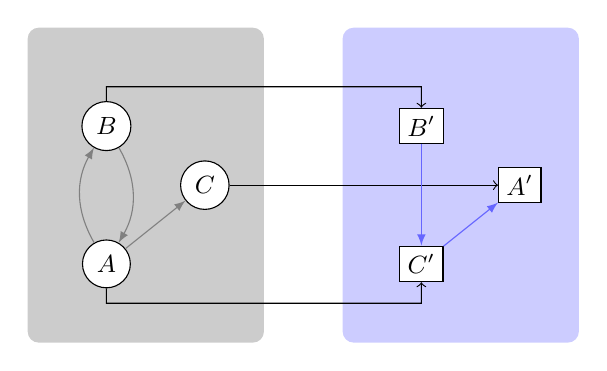
\begin{tikzpicture}
			\fill[rounded corners, gray!40] (0,0) rectangle (3,4);
			\fill[rounded corners, blue!20] (4,0) rectangle ++(3,4);
			%--
			\node[fill=white,inner sep=1mm,circle, draw, font=\small] (A) at (1,1) {\(A\)};
			\node[fill=white,inner sep=1mm,circle, draw, font=\small] (B) at (1,2.75) {\(B\)};
			\node[fill=white,inner sep=1mm,circle, draw, font=\small] (C) at (2.25,2) {\(C\)};
			\begin{scope}[xshift=4cm]
				\node[fill=white,inner sep=1mm, draw, font=\small] (A') at (1,1) {\(C'\)};
				\node[fill=white,inner sep=1mm, draw, font=\small] (B') at (1,2.75) {\(B'\)};
				\node[fill=white,inner sep=1mm, draw, font=\small] (C') at (2.25,2) {\(A'\)};
			\end{scope}
			\draw[->] (A) |- ++(4,-.5) -- (A');
			\draw[->] (B) |- ++ (4,.5) -- (B');
			\draw[->] (C) -- (C');
			%--
			\draw[-latex,gray] (A) -- (C);
			\draw[-latex,blue!60] (A') -- (C');
			\draw[-latex,gray] (A) to[bend left] (B);
			\draw[-latex,gray] (B) to[bend left] (A);
			\draw[-latex,blue!60] (B') -- (A');
		\end{tikzpicture}
	\end{center}
	\caption{\Todo{captione}}
\end{figure}
Le componenti \(A,B,C,\dots\) però ora non sono parte del discorso in un linguaggio naturale; sono `elementi' di una collezione --spesso gigantesca: \emph{tutti} i gruppi, \emph{tutte} le varietà differenziabili, senza eccezione-- \(\mathcal{L}\), che si chiamerà una `categoria'; Carnap definisce un funtore come una relazione funzionale tra linguaggi, che `preserva l'analisi logica'; per noi, un funtore è una relazione funzionale tra linguaggi, che preserva, in qualche modo da determinare, le relazioni che sussistono tra le loro diverse parti.

In questo senso la nozione data da Mac Lane ed Eilenberg in \cite{gtone} stava fondando un approccio \emph{relazionale}, dinamico, alla costruzione e alla comprensione degli oggetti matematici: le strutture non esistono di per loro, ma in una rete di relazioni, separate dalle quali esse sono incomprensibili, o comprensibili con maggiore fatica intellettuale.\footnote{H. Poincaré, il nonno della teoria delle categorie, disse che `la matematica non è solo un insieme di teoremi, così come una casa non è solo un mucchio di mattoni'. In maniera un po' più poetica (si veda il testo di Cook \cite{Cook1977-ry}) nella mitologia vedica, quando Indra immagina il mondo lo costruisce come una ragnatela o rete, in ciascuno dei cui nodi viene posto un gioiello; ogni \emph{dharma}, cioè ogni concetto sensibile o immaginabile, sia esso passato presente o futuro, è un nodo in questa rete, e la superficie di ciascun gioiello riflette ogni altro, cosicché ogni cosa che esiste implica tutte le altre (secondo il principio detto \emph{pratītyasamutpāda}, letteralmente traducibile come \emph{mutua produzione condizionata}).

	Il libro che leggete ora non è il luogo adatta ad approfondire la questione dal punto di vista storico o filosofico (e ancor meno lo è questa introduzione); chi legge consulti \cite{marquis, kromer} per dei testi introduttivi sulla storia della teoria delle categorie --apprenderà lì che la teoria delle categorie ha molti precursori, che si possono far risalire molto più indietro nel tempo del 1945, anno della pubblicazione di \cite{gtone}. Un esempio su tutti, il cosiddetto \emph{programma di Erlangen} proposto da Klein in una famosa prolusione del 1872, \cite{Klein1893}.}

\medskip
Lo scopo di questa introduzione non è delineare una storia completa della teoria delle categorie; chi legge troverà nel libro di Kr\"omer \cite{kromer} un esempio già insuperabile, che è pienamente un testo \emph{di matematica}. La teoria delle categorie è ubiquitaria in ciò che la logica, l'algebra, la geometria moderna è stata dal secondo dopoguerra, tanto che è inestricabile dalla storia della matematica del ventesimo secolo, che è vasta e ancora in via di definizione; delineare questa storia non compete certamente a noi che la stiamo vivendo.

Il punto che vogliamo rendere esplicito qui ed ora è che fare quindi della teoria delle categorie una disciplina eminentemente astratta, che mal tollera motivazioni concrete dietro le definizioni --tali motivazioni sono sempre radicate nell'esperienza sensibile, solo talvolta un po' meno direttamente-- tradisce completamente la verità storica.

All'esatto contrario, lo spirito che ha animato la teoria delle categorie è quello di una comunità di matematici che hanno tentato indefessamente di spiegare in termini di pochi e semplici concetti essenziali la natura e il comportamento di costruzioni matematiche che a prima vista erano del tutto scorrelate tra loro: è stata edificata secondo scelte stilistiche che nella loro apparente ingenuità hanno dato diversi frutti. Senza nessuna pretesa di completezza o di autorità, proviamo a descrivere quali sono queste idee.
\begin{itemize}
	\item Gli assiomi che fondano una teoria devono essere pochi e ben motivati, vuoi dall'esperienza sensibile, vuoi dal numero elevato di esempi vantaggiosi che \emph{quegli} assiomi, e non altri, riescono a descrivere. Al di fuori della teoria delle categorie, la teoria della misura è un esempio relativamente buono di questo tipo di ragione.\footnote{Un famoso teorico delle categorie, J. Bénabou, produce un `cattivo esempio' che riportiamo senza pretesa di essere letterali (e soprattutto senza voler offendere nessuno): per costruire l'insieme delle coppie ordinate \((a,b)\) a partire da due insiemi \(A,B\) è necessario, formalmente parlando, considerare l'insieme \(2^{2^{A\cup B}}\), per poi restringere il discorso alle coppie di una certa forma ben precisa: la coppia ordinata \((a,b)\) consta dell'insieme \(\{\{a\},\{a,b\}\}\). In particolare, per considerare il prodotto cartesiano \(\mathbf{N} \times \mathbf{N}\) di due copie dei naturali (insieme di cui \emph{certamente} vogliamo essere in grado di parlare), va considerato l'insieme \(2^{2^{\mathbf{N} \cup \mathbf{N}}}\): insieme che è gigantesco, e Bénabou definisce `aberrante' la pratica di doverlo considerare per parlare di un oggetto tanto semplice quanto quello che contiene elementi tanto semplici quanto le coppie \((15,18), (3,7), (12, 259)\dots\)

		      In teoria delle categorie, invece, il prodotto cartesiano \(A\times B\) è definito in maniera molto più snella, e non meno rigorosa.}
	\item La matematica deve essere ispirata a un principio di ergonomia e modularità; deve essere relativamente semplice e intuitivo maneggiare gli enti che compongono una teoria, e deve essere chiaro come poter esportare alcuni suoi frammenti a un contesto diverso: che differenza c'è, in ultima istanza, tra un monoide, un anello, e un gruppo dove le operazioni di moltiplicazione e inversione sono continue rispetto a una topologia? In questo senso, la matematica deve essere ispirata a un canone simile a quello che orienta la scrittura di `buon' codice sorgente quando si programma. Tutti sono capaci di scrivere una funzione che calcola un fattoriale; già meno persone sono capaci di farlo tenendo d'occhio il costo computazionale, la leggibilità, la mantenibilità della teoria/libreria dove quel teorema/codice è immerso.
	\item Quando teorie diverse possiedono dei tratti comuni, esiste una spiegazione profonda, non accidentale, per questo. Lo scopo --o l'effetto-- di una parte piuttosto vasta di teoria delle categorie è stato di trovare questa spiegazione profonda, renderla evidente e cercare di portarla alle sue estreme conseguenze. Le applicazioni maggiori di questo principio si possono apprezzare in `discipline dalla natura altamente dialettica' (una locuzione rubata a \cite{lawvere1999profilo}, una lettura squisita che invitiamo chi legge a reperire ad ogni costo), come la geometria e la logica; ma abbondano anche gli esempi in algebra astratta (vedremo questa idea in azione proprio quando cercheremo di `spiegare' il motivo per cui tutti i teoremi di isomorfismo si somigliano tra loro).
	      % \item La matematica possiede un certo grado di auto-referenzialità: le teorie matematiche si possono apprezzare come un certo tipo particolare di oggetto matematico, che può essere compreso mediante il linguaggio matematico. Lungi dall'essere una fumosa affermazione filosofica, questa idea viene sostanziata mediante il linguaggio delle categorie.
\end{itemize}
L'opinione di noi che scriviamo è che questo punto di vista, al di là dei suoi meriti concreti, misurabili, confermi come lo scibile matematico sia alla portata di chiunque lo voglia cogliere, quando esso sia espresso in termini di pochi concetti fondamentali.

Quei concetti riusciranno poi a delineare cosa, all'interno delle verità del linguaggio, è una tautologia, e concentrare le proprie energie sul comprendere appieno ciò che non lo è. Se è vero che il discente paga un prezzo all'ingresso, perché non deve solo imparare definizioni e teoremi e tecniche di calcolo, ma soprattutto un modo di pensare diversamente (e ripensare, e ripensare ancora) a cosa è la matematica e al contempo \emph{disimparare} alcune abitudini, i rudimenti del linguaggio categoriale rendono più semplice, veloce ed efficiente apprezzare la natura intima di definizioni molto diverse tra loro, nate per risolvere problemi diversi, e sviluppate in dialetti diversi.

Questo ha un costo cognitivo non indifferente: una indole poliedrica, e poco affine alla specializzazione, aiutano ad apprendere lo spirito dietro molte definizioni; ma questa indole, senza delle abilità di risolutore di problemi, rende impossibile \emph{fare i conti} adoperando le definizioni apprese.

\medskip
Lo scopo del libro che avete in mano è anche colmare questo abisso tra idee profonde, di ispirazione filosofica, generalista ed evocativa, e la natura eminentemente pratica (e quindi frustrante, pedissequa, quasi noiosa) del ragionamento matematico.

Ben più di una certa cattiva divulgazione, noi crediamo che questo approccio riesca a mostrare che la matematica è `alla portata di tutti', e secondo noi colpendo certamente più al cuore di alcuni tentativi.

\medskip
Esso nasce però anche con un fine molto più immediato: accompagnare un corso di teoria delle categorie che, durante l'anno accademico 2021-22 si è svolto online, su youtube, tenuto dal gruppo ItaCa (\url{https://progetto-itaca.github.io/pages/course.html}). Gli autori del libro sono i docenti di quel corso a cui abbiamo deciso di dare il nome collettivo di \emph{Outis} (\(O\tilde{\acute\upsilon}\tau\iota\varsigma\), Nessuno, è il nome con cui Ulisse ingannò Polifemo; ci piaceva, o meglio piaceva a uno degli autori, che questo libro fosse stato scritto da Nessuno).\footnote{Non menzionare nemmeno una volta i loro nomi sarebbe irrispettoso; appaiono qui, quasi invisibili, una volta sola:
	Greta Coraglia, Jacopo Emmenegger, Enrico Ghiorzi, Francesca Guffanti, Fosco Loregian, Beppe Metere, Daniele Palombi e Paolo Perrone.}

Ci ha spinto a impegnarci in questa ulteriore fatica il fatto che, con poche eccezioni, agli atenei italiani manca un corso il cui argomento principale sia la teoria delle categorie; solitamente si apprendono i suoi rudimenti perché è necessario introdurre delle costruzioni in geometria algebrica, algebra omologica, teoria degli anelli (e, sebbene molto raramente, in analisi).

Manca, invece, un corso che `riordini' le nozioni matematiche del discente unificandole sotto i pochi e fondamentali concetti della matematica strutturale. Questo è lo scopo concreto del libro che avete in mano.

\medskip
Come è strutturato, quindi, questo libro? E' innanzitutto suddiviso in capitoli, che rispecchiano la struttura del corso ma lo espandono laddove sia necessario (ad esempio, vi sono costruzioni ed esempi nel libro che non troverete a lezione; il capitolo \ref{cap:fattorizzazione} non è presente nel corso, eccetera); le sezioni di ogni capitolo si concludono con degli esercizi per il lettore, solitamente 3-5 per sezione. Gli esercizi sono risolti alla fine del libro, in una appendice; la ragione è che dopo i primi anni di studio della matematica, raramente si impiega un po' di tempo per mostrare agli studenti come si fanno gli esercizi, o per essere più precisi, quali sono le tecniche che il vecchio matematico, che le ha affinate con l'esperienza, sa essere valide per fare una dimostrazione. Non avere questo tipo di conferma della correttezza dei propri argomenti, o averlo solo dietro enorme insistenza, è molto castrante quando oltre a imparare definizioni, teoremi e corollari ci si trova a dover imparare un nuovo modo di ragionare.

Chi legge si accorgerà leggendo le soluzioni degli esercizi (ma dovrebbe farlo solo dopo aver provato a risolverli!) che esistono alcune tattiche di dimostrazione stabilite, che possono essere descritte in poche parole e che hanno un ampio campo di validità. Queste tecniche spesso si aiutano l'un l'altra.
\Todo{}
\medskip
Concludiamo questa introduzione parlando, finalmente, di matematica in senso stretto.

Lo scopo delle brevi sezioni che seguono e che chiudono il capitolo è di presentare quattro `preludi' categoriali, raccolti dai vari àmbiti del bagaglio culturale di uno studente che è alla fine di una laurea triennale in una generica università italiana.

L'accento, per ora, non è sul rigore, ma sul giusto grado di espressività e generalità.
\section*{Abelianizzazione, o `naturalità'}
Consideriamo un gruppo \(G\), la cui operazione è denotata moltiplicativamente; in esso, consideriamo il sottogruppo generato dagli elementi della forma
\[[x,y]:= xyx^{-1}y^{-1}\]
al variare di \(x,y\in G\). Si tratta quindi del sottogruppo i cui elementi sono generati dai `commutatori' della forma
\[t = [x_1,y_1][x_2,y_2]\cdots[x_n,y_n]\]
al variare di \(x_i,y_i\in G\) e \(n\ge 0\) in \(\mathbf{N}\) (se \(n=0\), il prodotto è vuoto e quindi l'elemento in questione è uguale all'identità di \(G\)): è infatti facile vedere che l'inverso \([x,y]^{-1}\) di un commutatore è a sua volta un commutatore.

\`E altresì facile mostrare che il sottogruppo \([G,G]\) è normale in \(G\), e che è il sottogruppo minimale con la proprietà che il quoziente \(G/[G,G]\) è abeliano (cioè, se \(N\) è normale e \(G/N\) è abeliano, allora \(N\) contiene \([G,G]\)).

Il gruppo \(G/[G,G]\) prende il nome di \emph{abelianizzato} di \(G\), si denota a volte con \(G^\text{a}\), e soddisfa la seguente proprietà di \emph{universalità}:
\begin{quote}
	Esiste un unico omomorfismo \(\alpha : G \to G^\text{a}\) con la seguente `proprietà universale': per ogni omomorfismo di gruppi \(f : G \to A\), di codominio un gruppo abeliano \(A\), esiste un unico omomorfismo di gruppi \(\bar f : G^\text{a} \to A\) con la proprietà che \(\bar f \circ \alpha = f\).
\end{quote}
\begin{remark}
	Si può pensare a \(G\mapsto G^\text{a}\) come ad una `costruzione' che ad un gruppo \(G\) associa un altro gruppo \(G^\text{a}\), definito da una certa proprietà; questa associazione è poi responsiva al fatto che tra gruppi distinti \(G,H\) possono esistere degli omomorfismi \(f : G \to H\), nel senso che segue:
	\begin{quote}
		Dato un omomorfismo di gruppi \(f : G \to H\) esiste un omomorfismo \(f^\text{a} : G^\text{a} \to H^\text{a}\) tra gli abelianizzati di \(G,H\), definito mandando una classe di equivalenza \(g\cdot [G,G]\) in \(f(g)\cdot [H,H]\).
	\end{quote}
	L'unica cosa da verificare è che \(f^\text{a}\) così definita sia veramente una funzione; del resto, \(f\) discende al quoziente \(G^\text{a}\) partendo da una funzione \(\tilde f : G\to H^\text{a}\), cosa che segue immediatamente dal fatto che \(f\) manda \([G,G]\) in \([H,H]\) (perché \(f[x,y]=[fx, fy]\in [H,H]\)).
\end{remark}
Vi sono due proprietà che ora la corrispondenza \(f\mapsto f^\text{a}\) soddisfa: la loro verifica è a dir poco immediata.
\begin{enumtag}{fu}
	\item \label{fct_1} Se \(1_G\) è l'omomorfismo identico di un gruppo \(G\), allora \(1_G^\text{a}\) è l'omomorfismo identico di \(G^\text{a}\).
	\item \label{fct_2} Considerando due omomorfismi di gruppi componibili \(u : G\to H, v : H\to K\), si ha che
	\[(v\circ u)^\text{a} = v^\text{a} \circ u^\text{a}\]
	(l'uguaglianza di funzioni è una uguaglianza \emph{estensionale}, cioè valida elemento per elemento).
\end{enumtag}
Nelle stesse notazioni, si osservi anche che la definizione di \(f^\text{a} : G^\text{a} \to H^\text{a}\) è l'unica possibile qualora si chieda che \(f^\text{a}(\pi^G(x)) = \pi^H(f(x))\) per ogni \(x\in G\), ossia che il diagramma di omomorfismi
\[\xymatrix{
	G \ar[r]^-{\pi^G} \ar[d]_f & G^\text{a}\ar[d]^{f^\text{a}} \\
	H \ar[r]_-{\pi^H} & H^\text{a}
	}\]
sia commutativo.

La famiglia di omomorfismi \(\{\pi^G : G\to G^\text{a}\}\) è quindi specificata in maniera `uniforme' nel parametro da cui dipende, ossia è determinata, per un qualsiasi gruppo \(G\), dalla proiezione al quoziente \(\pi^G : G\to G/[G,G] : x\mapsto x\cdot[G,G]\) che manda un dato elemento nella sua classe laterale. In altre parole (meno precise, ma forse più evocative) per \emph{ogni} gruppo \(G\) è possibile costruire una funzione \(\pi^G : G\to G/[G,G]\), definita sempre alla stessa maniera in dipendenza di \(G\), in maniera tale che il quadrato precedente sia commutativo.

In situazioni simili, diciamo che l'assegnazione \(G\mapsto (\pi^G : G\to G^\text{a})\) è \emph{naturale}, o più precisamente che \(\pi^G\) è (la componente di) una \emph{trasformazione naturale}
\[\xymatrix{\boldsymbol\pi  : (\_) \ar@{=>}[r] & (\_)^\text{a}.}\]
Il dominio e il codominio di una trasformazione naturale sono dei \emph{funtori}: non daremo qui la definizione (che seguirà in \ref{sec_funtori}), ma l'idea che chi legge dovrebbe trattenere è che sappiamo trasformare un gruppo \(G\) in un altro gruppo \(F(G)\), e ogni omomorfismo di gruppi \(f : G\to H\) in un omomorfismo \(F(f) : F(G)\to F(H)\), in modo tale che le condizioni \ref{fct_1} e \ref{fct_2} siano verificate: quindi,
\begin{enumerate}
	\item Se \(1_G\) è l'omomorfismo identico, allora \(F(1_G)\) è l'omomorfismo identico di \(F(G)\).
	\item Considerando due omomorfismi componibili \(u : G\to H, v : H\to K\), si ha che
	      \[F(v\circ u) = Fv \circ Fu.\]
\end{enumerate}
In questo caso specifico, il dominio di \(\boldsymbol\pi\) è il funtore \emph{identico} definito in modo tautologico; il codominio è il funtore di abelianizzazione, la cui funtorialità è chiara grazie a \ref{fct_1} e \ref{fct_2}.
% \begin{remark}
% 	L'idea intuitiva che questa sezione vuole comunicare è che tutte le proprietà matematiche di una certa importanza si possono rifrasare nello stesso modo; la costruzione che produce \(G^\text{a}\) è un esempio particolare di una pratica generale, quella di definire un oggetto matematico mediante una certa \emph{proprietà universale}, che cioè somigli alla proprietà di \(G^\text{a}\).

% 	Siamo posti di fronte al problema di costruire un oggetto con certe proprietà. Se (è possibile trovarlo e) una volta che lo si è costruito esso soddisfa un requisito di universalità (che superficialmente cambia di volta in volta, ma che a conti fatti chiede sempre la stessa cosa: per ogni `diagramma' della tal forma, esiste un \emph{unico} omomorfismo della tale altra forma, per cui\dots), esso è \emph{univocamente determinato} da questa proprietà.
% \end{remark}
% \`E ora conveniente pensare agli omomorfismi di gruppo --e in effetti, relativi a qualsiasi altra struttura: i gruppi non hanno niente di speciale qui-- come `deformazioni' di una struttura di tipo \(G\) in una di tipo \(H\). In questo senso, l'assegnazione \(G\mapsto G^\text{a}\) è speciale in due sensi: prima di tutto, ogni gruppo \(G\) ha un omomorfismo canonico \(\pi_G : G \to G^\text{a}\) di proiezione al quoziente; secondo, per ogni \(f : G \to H\) le condizioni sopra sono verificate.
\section*{Teoremi di isomorfismo, o `universalità'}
I teoremi di isomorfismo nelle diverse strutture dicono tutti la stessa cosa
\section*{Completamenti, o `aggiunzioni'}
Dato uno spazio metrico \((X,d)\) una \emph{successione di Cauchy} è una successione \(a : \bbN \to X\) tale che per ogni \(\epsilon>0\) esiste un \(N\gg 1\) per cui
\[\forall n,m> N\; : \; d(a_n,a_m) < \epsilon.\]
Dato \((X,d)\) è sempre possibile costruire uno spazio metrico `completo' \(\bar X\) che contiene \(X\) come un sottospazio isometrico e tale che ogni successione \(a : \bbN \to \bar X\) che sia di Cauchy è convergente.

Questo spazio soddisfa la seguente proprietà: comunque sia dato uno spazio metrico completo \((Y,d_Y)\) e una mappa nonespansiva \(f : X\to Y\), esiste un'unico modo di estendere \(f\) a una mappa nonespansiva \(f^* : \bar X \to Y\) che coincide con \(f\) su \(X\le \bar X\).

Per costruire \(\bar X\), consideriamo lo spazio \((C^0(X,\bbR),d_\infty)\) delle funzioni continue \(X\to\bbR\), dotato della metrica unifome \((f,g)\mapsto \sup_x |fx-gx|\), che è facile mostrare è uno spazio metrico completo. Allora l'embedding \(j : X\mono \bar X\) è dato dalla funzione che manda \(x\) in \(\bar x = d(x,-) : X\to \bbR\), la quale è continua (e iniettiva, dato che la metrica è non degenere); dalla disuguaglianza triangolare segue che \(\sup_z|\bar{x}(z)-\bar{y}(z)|\le d(x,y)\) e in effetti vale l'uguaglianza, ponendo \(z=x\); ma allora, \(j : X\mono \bar X\) è una isometria.

Lo spazio così costruito
\section*{Il teorema di Brouwer, o `funtorialità'}
Dimostrare una cosa difficile `muovendo le mani'
\begin{exercises}
\item \label{ex_prelude_1} un exercise sul primo preludio
\item \label{ex_prelude_2} un exercise sul secondo preludio
\item \label{ex_prelude_3} Mostrare che \(j : X\to \bar X\) costruito in \autoref{} ha immagine densa; mostrare che \(\bar X\) è effettivamente tale che ogni successione di Cauchy converge; mostrare che il sottospazio \(j(X)\) è denso in \(\bar X\), ossia che ogni elemento \(f\) di \(\bar X\) è il limite \(\lim_n f_n\) di una successione di elementi della forma \(f_n=\bar x_n^f\)

Si riesce a costruire esplicitamente un'isometria \((\bbR, |\_|) \cong (C^0(\bbQ,\bbR), d_\infty)\)?
\item \label{ex_prelude_4} un exercise sul quarto preludio
\end{exercises}
